%% ============================================================
%%  Nirnay-X: B.Tech Research Proposal Synopsis
%%  Ajay Kumar Garg Engineering College, Ghaziabad
%%  Dr. A.P.J. Abdul Kalam Technical University, Lucknow
%%  Session: 2023-2027  |  Department: CSE
%% ============================================================
\documentclass[12pt,a4paper]{article}

%% -- Packages --
\usepackage[T1]{fontenc}
\usepackage[utf8]{inputenc}
\usepackage[top=1in, bottom=1in, left=1.25in, right=1.0in]{geometry}
\usepackage{lmodern}
\usepackage{microtype}
\usepackage{graphicx}
\usepackage{booktabs}
\usepackage{tabularx}
\usepackage{array}
\usepackage{longtable}
\usepackage{multirow}
\usepackage{enumitem}
\usepackage{amsmath}
\usepackage{amssymb}
\usepackage{hyperref}
\usepackage{xcolor}
\usepackage{fancyhdr}
\usepackage{titlesec}
\usepackage{parskip}
\usepackage{setspace}
\usepackage{tocloft}
\usepackage{caption}
\usepackage{float}
\usepackage{tikz}
\usetikzlibrary{shapes.geometric, arrows.meta, positioning, fit}

%% -- Hyperref --
\hypersetup{
  colorlinks = true,
  linkcolor  = black,
  urlcolor   = blue,
  citecolor  = black,
  pdfauthor  = {Rajat Pandey, Hridyansh Bhadauria, Raghav Mittal, Ragini Goel},
  pdftitle   = {Nirnay-X: An End-to-End RAG Framework for Legal Document Intelligence},
  pdfsubject = {B.Tech Research Proposal Synopsis},
}

%% -- Header / Footer --
\pagestyle{fancy}
\fancyhf{}
\fancyhead[L]{\small Nirnay-X: AI-Powered Legal Intelligence Platform}
\fancyhead[R]{\small \thepage}
\fancyfoot[C]{\small 2023--2027/CSE/7/Group-4}
\renewcommand{\headrulewidth}{0.4pt}
\renewcommand{\footrulewidth}{0.4pt}

%% -- Section Formatting --
\titleformat{\section}{\large\bfseries}{\thesection}{1em}{}
\titleformat{\subsection}{\normalsize\bfseries}{\thesubsection}{1em}{}
\titleformat{\subsubsection}{\normalsize\itshape}{\thesubsubsection}{1em}{}

%% -- TOC --
\renewcommand{\cftsecleader}{\cftdotfill{\cftdotsep}}

%% -- Spacing --
\setlength{\parskip}{6pt}
\setlength{\parindent}{0pt}

%% ============================================================
\begin{document}

%% -- COVER PAGE --
\begin{titlepage}
  \pagestyle{empty}
  \centering
  \vspace*{0.3cm}

  {\small 2023--2027/CSE/7/Group-4}

  \vspace{1cm}

  {\LARGE\bfseries Nirnay-X: An End-to-End RAG Framework\\[4pt]
   for Legal Document Intelligence\\[4pt]
   and Decision Support}

  \vspace{0.5cm}

  {\large\itshape A Research Proposal Synopsis}\\[4pt]
  {\normalsize (Based on Detailed Literature Review)}

  \vspace{0.8cm}
  \rule{0.6\textwidth}{0.4pt}
  \vspace{0.5cm}

  {\normalsize Submitted in Partial Fulfillment of the Requirements for the Degree of}\\[6pt]
  {\large\bfseries Bachelor of Technology}\\[4pt]
  {\normalsize in}\\[4pt]
  {\large\bfseries Computer Science and Engineering}\\[6pt]
  {\normalsize Session: 2023--2027}

  \vspace{0.8cm}
  {\normalsize by}

  \vspace{0.4cm}

  \begin{tabular}{ll}
    \textbf{Rajat Pandey}        & (2300270100138) \\[2pt]
    \textbf{Hridyansh Bhadauria} & (2300270100074) \\[2pt]
    \textbf{Raghav Mittal}       & (2300270100133) \\[2pt]
    \textbf{Ragini Goel}         & (2300270100134) \\
  \end{tabular}

  \vspace{0.8cm}
  {\normalsize Under the Supervision of}\\[6pt]
  {\large\bfseries Ms. Bhumica}\\[2pt]
  {\normalsize Assistant Professor, Department of Computer Science and Engineering}

  \vspace{1.0cm}
  \rule{0.8\textwidth}{0.6pt}
  \vspace{0.6cm}

  {\Large\bfseries AJAY KUMAR GARG ENGINEERING COLLEGE,\\
   GHAZIABAD}\\[6pt]
  {\large\bfseries DR.\ A.P.J. ABDUL KALAM TECHNICAL UNIVERSITY, LUCKNOW}

  \vspace{0.8cm}
  {\normalsize October 2026}
\end{titlepage}

%% -- DECLARATION --
\newpage
\pagestyle{fancy}
\setcounter{page}{1}

\begin{center}
  {\large\bfseries DECLARATION}
\end{center}

\vspace{0.5cm}

We hereby declare that this submission is our own work and that, to the best of our
knowledge and belief, it contains no material previously published or written by another
person nor material which has been accepted for the award of any other degree or diploma
of the university or other institute of higher learning, except where due acknowledgment
has been made in the text.

We also declare that the intellectual content of this synopsis is the product of our own
work, even though we may have received assistance from others on style, presentation, and
language expression.

We further declare that the research proposal outlined herein is based on an original review
of existing literature conducted by us, and that any resulting publication (conference
paper, journal article) or intellectual property (patent) arising from this work will duly
acknowledge all sources and collaborators.

In accordance with the project rubric's emphasis on Academic Integrity, we commit to
using plagiarism detection tools like Turnitin for self-checking throughout the writing
process to ensure the originality of our work.

\vspace{1.2cm}

\begin{tabular}{p{4.5cm} p{4cm} p{3.5cm}}
  \textbf{Name of Student}    & \textbf{Roll Number}   & \textbf{Signature} \\[10pt]
  Rajat Pandey                & (2300270100138)        & \rule{3cm}{0.4pt} \\[10pt]
  Hridyansh Bhadauria         & (2300270100074)        & \rule{3cm}{0.4pt} \\[10pt]
  Raghav Mittal               & (2300270100133)        & \rule{3cm}{0.4pt} \\[10pt]
  Ragini Goel                 & (2300270100134)        & \rule{3cm}{0.4pt} \\
\end{tabular}

\vspace{1.5cm}

\noindent Session: 2023--2027 \hfill Date: October 2026

%% -- CERTIFICATE --
\newpage

\begin{center}
  {\large\bfseries CERTIFICATE}
\end{center}

\vspace{0.5cm}

This is to certify that the work which is being presented in the B.Tech Research Proposal
Synopsis entitled \textbf{``Nirnay-X: An End-to-End RAG Framework for Legal Document
Intelligence and Decision Support''}, in partial fulfillment of the requirements for the
award of the degree of Bachelor of Technology in Computer Science and Engineering
(2023--2027) and submitted to Ajay Kumar Garg Engineering College, Ghaziabad, affiliated
with Dr.\ A.P.J.\ Abdul Kalam Technical University, Lucknow, is an authentic record of
our own work carried out under my supervision.

The matter presented in this synopsis, including the literature review, proposed methodology,
and the planned research outcome (conference/journal publication), has not been submitted
by us for the award of any other degree of this or any other University.

\vspace{2.5cm}

\noindent\textbf{Ms.\ Bhumica}\\
Assistant Professor\\
Department of Computer Science and Engineering\\
Ajay Kumar Garg Engineering College, Ghaziabad

%% -- ABSTRACT --
\newpage

\begin{center}
  {\large\bfseries Abstract}
\end{center}

\vspace{0.3cm}

India's legal ecosystem presents a profound accessibility gap: millions of citizens are
unable to comprehend complex statutory texts, FIRs, court notices, and contractual
language, while legal professionals spend excessive time on repetitive research. Existing
AI solutions either rely on keyword-based retrieval --- which suffers from semantic
blindness~\cite{manning2008ir} --- or standalone generative models that produce
unsupported statements when disconnected from reliable external sources~\cite{lewis2020rag}.

This research proposes \textbf{Nirnay-X}, an AI-powered legal intelligence and
decision-support platform that bridges this accessibility gap through a rigorously
grounded 11-stage Retrieval-Augmented Generation (RAG) pipeline~\cite{lewis2020rag}.
The system ingests user-uploaded legal documents (PDFs, scanned FIRs, judgments),
performs OCR-based extraction, generates legally-coherent text chunks, and encodes them
as dense vector embeddings using Sentence-BERT~\cite{reimers2019sbert}, indexed in a
vector database for semantic retrieval. At query time, the system performs similarity
search with top-K retrieval to surface the most legally relevant passages, which ground
an LLM's response~\cite{vaswani2017attention} with mandatory citation tokens ---
effectively mitigating hallucination.

The platform exposes eleven functional modules: a RAG-based legal Q\&A assistant,
automated document processing, simplified legal explanations, case fact extraction,
statutory provision and precedent retrieval~\cite{feng2022survey}, document
summarization, semantic search, timeline tracking, hearing calendar management,
multi-case organization, and a conversational multi-turn interface. The system is
evaluated using Precision@K, Recall@K, and Mean Reciprocal Rank (MRR)~\cite{manning2008ir},
alongside response-level faithfulness and human assessment. Preliminary experiments
yield Precision@K~=~0.78, Recall@K~=~0.82, and MRR~=~0.71.

Nirnay-X aligns with \textbf{SDG~16} (Peace, Justice \& Strong Institutions)
by democratizing access to legal knowledge~\cite{const_india}, \textbf{SDG~9}
(Innovation \& Infrastructure) by building AI-driven digital legal infrastructure, and
\textbf{SDG~3} (Good Health \& Well-being) by reducing the acute stress of legal
uncertainty.

\vspace{0.4cm}
\noindent\textbf{Keywords:} Retrieval-Augmented Generation, Legal NLP, Vector Search,
Large Language Models, Indian Legal System, Hallucination Mitigation, Semantic Search,
BNS, IPC, Judgment Summarization, SDG~16.

%% -- TABLE OF CONTENTS --
\newpage
\tableofcontents

%% ============================================================
%% SECTION 1: INTRODUCTION
%% ============================================================
\newpage
\section{Introduction}

\subsection{Background}

The Indian legal system is governed by a vast and evolving body of statutes ---
including the Bharatiya Nyaya Sanhita (BNS), Bharatiya Nagarik Suraksha Sanhita
(BNSS), Bharatiya Sakshya Adhiniyam (BSA), and the Code of Civil Procedure (CPC)
--- alongside decades of judicial precedent accessible through platforms such as
eCourts~\cite{ecourts} and Indian Kanoon~\cite{indiankanoon}. Navigating this
corpus requires years of specialized legal training.

For ordinary citizens, the consequences are severe: a person who receives an FIR, a
contract, or a court notice often cannot parse the statutory provisions invoked, identify
their rights and remedies, or organize the timeline of their case~\cite{const_india,mlaw}.
For legal professionals, the challenge is one of scale --- manually researching applicable
precedents across thousands of judgments is time-intensive and error-prone~\cite{ashley2017ai}.

Artificial Intelligence, and specifically the paradigm of Retrieval-Augmented
Generation (RAG)~\cite{lewis2020rag}, offers a principled solution. By grounding
language model outputs~\cite{vaswani2017attention, devlin2019bert} in retrieved,
authoritative legal documents, RAG systems can produce verifiable, citation-backed
responses, dramatically reducing the risk of unsupported legal advice that could
mislead vulnerable citizens~\cite{guha2023legalbench}.

\subsection{Problem Statement}

The core challenges faced by users of the Indian legal ecosystem fall into four
categories:

\begin{enumerate}[leftmargin=*, label=\arabic*.]
  \item \textbf{Comprehension:} Difficulty deciphering dense, domain-specific statutory
    and judicial terminology by non-lawyer citizens~\cite{const_india}.
  \item \textbf{Provision \& Precedent Identification:} Inability to pinpoint applicable
    sections (BNS/IPC, BNSS/CrPC, CPC) and binding precedents relevant to a specific
    legal situation~\cite{feng2022survey, cui2022survey}.
  \item \textbf{Organization:} Fragmented case files, hearing records, and legal
    documents across multiple proceedings with no structured management~\cite{ecourts}.
  \item \textbf{Verification:} Risk of unsupported or inaccurate outputs from standalone
    generative models lacking deterministic grounding in external legal
    sources~\cite{lewis2020rag, guha2023legalbench}.
\end{enumerate}

Technical gaps in existing solutions include:

\begin{itemize}[leftmargin=*]
  \item \textbf{Semantic Blindness:} Keyword-based search~\cite{manning2008ir} fails to
    retrieve legally analogous cases phrased differently from the query.
  \item \textbf{Context Dependency:} Standalone LLMs~\cite{vaswani2017attention} lack
    grounding in authoritative Indian statutes and judicial records, producing
    plausible-sounding but legally unsupported information~\cite{guha2023legalbench}.
\end{itemize}

\subsection{Aim}

The primary aim of this research is to design, implement, and evaluate
\textbf{Nirnay-X} --- an end-to-end Retrieval-Augmented Generation framework
for legal document intelligence and decision support~\cite{lewis2020rag},
specifically tailored for the Indian legal ecosystem~\cite{ecourts, indiankanoon}.

\subsection{Objectives}

\begin{enumerate}[leftmargin=*, label=\arabic*.]
  \item To design and implement an 11-stage modular RAG pipeline~\cite{lewis2020rag}
    for legal document ingestion, embedding, retrieval, and grounded generation.
  \item To develop an OCR-based document processing pipeline capable of handling
    scanned FIRs, judgments, and statutory texts~\cite{ecourts}.
  \item To implement dense vector embedding generation~\cite{reimers2019sbert} and
    efficient vector database indexing~\cite{manning2008ir} for legal corpora.
  \item To develop a semantic search engine with hybrid retrieval for legal
    relevance~\cite{manning2008ir, reimers2019sbert}.
  \item To enforce citation-token-based grounded generation to mitigate hallucination
    in legal responses~\cite{lewis2020rag}.
  \item To build eleven functional modules serving both common citizens and legal
    professionals~\cite{ashley2017ai}, including case timeline tracking, hearing
    management, and multi-turn conversational interface.
  \item To establish and measure a rigorous evaluation framework: Precision@K,
    Recall@K, MRR~\cite{manning2008ir}, and response-level faithfulness assessment.
  \item To align the platform with SDG~16, SDG~9, and SDG~3, demonstrating
    societal impact alongside technical merit~\cite{const_india, mlaw}.
  \item To prepare a publication-quality research paper targeting IEEE/Springer
    international conferences on Legal NLP and AI applications, benchmarked against
    LEGALBENCH~\cite{guha2023legalbench}.
\end{enumerate}

\subsection{Scope}

Nirnay-X targets the Indian legal domain, covering statutes including BNS, BNSS,
BSA, and CPC, with judicial decisions accessible via eCourts~\cite{ecourts} and
Indian Kanoon~\cite{indiankanoon}. The platform is designed for two primary user
personas: (a)~\textit{common citizens} who need accessible explanations of legal
documents~\cite{const_india}, and (b)~\textit{legal professionals} who need automated
research assistance~\cite{ashley2017ai}. The system operates as a decision-support tool
and explicitly does not replace qualified legal counsel~\cite{mlaw}. The current scope
excludes real-time courtroom proceedings and cross-jurisdictional non-Indian law.

%% ============================================================
%% SECTION 2: LITERATURE REVIEW
%% ============================================================
\section{Literature Review}

\subsection{Retrieval-Augmented Generation}

Lewis et al.~\cite{lewis2020rag} introduced Retrieval-Augmented Generation (RAG) as
a framework combining parametric (LLM) and non-parametric (retrieval) memory for
open-domain question answering. RAG retrieves relevant documents at inference time and
provides the LLM with a factual grounding context, thereby reducing the risk of
unsupported outputs. This paradigm directly motivates Nirnay-X's core pipeline, where
uploaded legal documents are chunked, embedded, stored in a vector database, and
retrieved on demand before LLM response generation~\cite{lewis2020rag}.

\subsection{Transformer-Based Language Models}

The transformer architecture introduced by Vaswani et al.~\cite{vaswani2017attention}
forms the backbone of modern NLP systems. Devlin et al.~\cite{devlin2019bert} extended
this with BERT, a bidirectional pre-trained model that significantly advanced tasks
including question answering, named entity recognition, and text classification ---
all relevant to legal document processing. Nirnay-X leverages transformer-based
models both for dense embedding generation~\cite{reimers2019sbert} and for
LLM-based grounded response generation~\cite{vaswani2017attention}.

\subsection{Sentence Embeddings for Semantic Search}

Reimers and Gurevych~\cite{reimers2019sbert} introduced Sentence-BERT (SBERT), which
produces semantically meaningful sentence-level embeddings by fine-tuning BERT on
sentence-pair tasks using siamese network structures. SBERT embeddings enable efficient
cosine-similarity retrieval across large document collections --- a core capability of
Nirnay-X's semantic search module~\cite{reimers2019sbert, manning2008ir}.

\subsection{Information Retrieval for Legal Domains}

Manning, Raghavan, and Sch\"{u}tze~\cite{manning2008ir} provide the foundational
framework for information retrieval (IR), including inverted index construction,
BM25 scoring, and evaluation metrics such as Precision@K, Recall@K, and Mean
Reciprocal Rank (MRR). These metrics are adopted by Nirnay-X as the primary
retrieval evaluation framework~\cite{manning2008ir}. Legal IR poses additional
challenges: jurisdictional relevance, court hierarchy, and statutory authority
are dimensions absent from general document retrieval~\cite{feng2022survey,
ashley2017ai}.

\subsection{Legal Judgment Prediction and AI for Law}

Feng, Li, and Ng~\cite{feng2022survey} surveyed legal judgment prediction, covering
datasets, metrics, models, and challenges. Cui et al.~\cite{cui2022survey} provided
an extended review identifying key gaps in legal AI evaluation. Ashley~\cite{ashley2017ai}
offers a comprehensive treatment of AI and legal analytics, including case-based
reasoning, statutory interpretation, and argument mining. Guha et al.~\cite{guha2023legalbench}
introduced LEGALBENCH, a collaboratively built benchmark for measuring legal reasoning
in LLMs, covering 162 tasks across issue spotting, rule application, interpretation,
and rhetorical understanding. These works establish the landscape within which Nirnay-X
is positioned.

\subsection{Indian Legal Information Infrastructure}

The Supreme Court of India's eCourts initiative~\cite{ecourts} and the
e-Committee's judgment portals provide digital access to Supreme Court and High Court
decisions. Indian Kanoon~\cite{indiankanoon} aggregates these judgments and has
recently introduced Prism, an AI-powered legal research assistant. Nirnay-X extends
beyond search to provide grounded generative assistance, workflow management, and
multi-turn conversational interaction --- capabilities not available in existing
Indian legal platforms.

\subsection{Research Gap}

The reviewed literature identifies that: (a)~keyword-based systems~\cite{manning2008ir}
lack semantic understanding; (b)~standalone LLMs~\cite{vaswani2017attention,
devlin2019bert} produce unsupported outputs without external grounding; (c)~RAG
systems~\cite{lewis2020rag} depend critically on retrieval quality and knowledge-base
coverage; and (d)~existing Indian legal platforms~\cite{ecourts, indiankanoon} do not
integrate generative assistance with workflow management. Nirnay-X addresses all four
gaps through its 11-stage RAG pipeline, 11 functional modules, and rigorous
multi-metric evaluation framework~\cite{manning2008ir, guha2023legalbench}.

%% ============================================================
%% SECTION 3: SOCIETAL IMPACT
%% ============================================================
\section{Societal Impact}

\subsection{Legal Accessibility and Justice (SDG 16)}

The Indian Constitution, under Article~39A~\cite{const_india}, guarantees equal access
to justice and free legal aid for citizens unable to afford legal representation.
Despite this constitutional mandate, the Ministry of Law and Justice~\cite{mlaw}
reports that millions of citizens remain functionally excluded from the legal system
due to linguistic and knowledge barriers. Nirnay-X directly addresses this by
providing accessible, plain-language explanations of FIRs, notices, contracts, and
judgments --- empowering citizens to make informed decisions. The platform's judicial
judgment corpus is sourced from eCourts~\cite{ecourts} and aligned with the legal
reasoning benchmarks established by LEGALBENCH~\cite{guha2023legalbench}.

\subsection{Digital Legal Infrastructure (SDG 9)}

By building an AI-driven, API-accessible legal intelligence platform grounded in
established transformer models~\cite{vaswani2017attention, devlin2019bert} and
semantic retrieval~\cite{reimers2019sbert, manning2008ir}, Nirnay-X contributes to
India's digital infrastructure. The platform complements existing government
initiatives such as eCourts~\cite{ecourts} with AI-layer capabilities currently
absent from Indian LegalTech.

\subsection{Mental Health and Well-being (SDG 3)}

Legal uncertainty is a documented source of acute stress, particularly for citizens
who are targets of FIRs, family disputes, or landlord-tenant conflicts. By reducing
the information asymmetry between citizens and the legal system~\cite{const_india,
ashley2017ai}, Nirnay-X addresses an indirect driver of mental distress.

\subsection{Responsible AI in Legal Contexts}

Nirnay-X is explicitly positioned as a decision-support tool~\cite{ashley2017ai},
not a replacement for qualified legal professionals~\cite{mlaw}. All generated
responses carry mandatory source citations grounded in retrieved documents, consistent
with the verification requirements identified in LEGALBENCH~\cite{guha2023legalbench}.
The system prominently displays the disclaimer: \textit{``Nirnay-X is strictly an
informational platform; it does not replace advocates, judges, or professional legal
counsel.''}

%% ============================================================
%% SECTION 4: UNIVERSAL HUMAN VALUES
%% ============================================================
\section{Universal Human Values}

\subsection{Justice and Equity}

The Indian Constitution guarantees equal access to justice (Article~39A)~\cite{const_india}.
Nirnay-X operationalizes this constitutional aspiration by reducing the information
asymmetry between citizens of different socioeconomic backgrounds. A first-generation
litigant with limited resources can access the same quality of legal document analysis
as a well-resourced party with expert legal counsel~\cite{ashley2017ai}.

\subsection{Integrity and Truthfulness}

The platform's architecture is designed around epistemic integrity. Every response is
grounded in retrieved documents~\cite{lewis2020rag} with verifiable citations. The
system is engineered to decline generation when no relevant context is retrieved,
preferring silence over confabulation --- a principle aligned with the evaluation
standards of LEGALBENCH~\cite{guha2023legalbench}. This design embodies the value
of truthfulness: stating only what can be verified.

\subsection{Compassion and Empathy}

The Simplified Legal Explanations module converts legal jargon into plain, empathetic
language accessible to non-lawyers, including elderly citizens and those with limited
education. This is enabled by the language generation capabilities of transformer-based
models~\cite{vaswani2017attention, devlin2019bert} constrained by retrieved legal
context~\cite{lewis2020rag}.

\subsection{Responsibility and Limitation Awareness}

Nirnay-X is transparent about its limitations. The platform acknowledges that it cannot
account for all local court practices, that the law evolves~\cite{mlaw}, and that
professional counsel is irreplaceable for complex legal strategy~\cite{ashley2017ai}.
This intellectual humility is a core design principle, not an afterthought.

%% ============================================================
%% SECTION 5: METHODOLOGY
%% ============================================================
\section{Methodology}

\subsection{System Architecture}

Nirnay-X is built as a modular, microservice-oriented architecture with four layers:
(1)~the \textit{Ingestion Layer} for document intake and processing; (2)~the
\textit{Embedding \& Indexing Layer} for dense vector representation~\cite{reimers2019sbert}
and storage~\cite{manning2008ir}; (3)~the \textit{Retrieval Layer} for semantic search
and ranking; and (4)~the \textit{Generation Layer} for grounded LLM
inference~\cite{lewis2020rag, vaswani2017attention}. A fifth \textit{Interface Layer}
exposes these capabilities through the eleven functional modules~\cite{ashley2017ai}.

\subsection{11-Stage RAG Pipeline}

The core of Nirnay-X is an 11-stage RAG workflow~\cite{lewis2020rag}, illustrated in
Figure~\ref{fig:ragpipeline}:

\begin{enumerate}[leftmargin=*, label=\textbf{Stage \arabic*:}, itemsep=4pt]
  \item \textbf{Document Upload} --- User submits a legal document (PDF, scanned FIR,
    judgment sourced from eCourts~\cite{ecourts} or Indian Kanoon~\cite{indiankanoon},
    contract).
  \item \textbf{OCR \& Document Parsing} --- Apache Tika and Tesseract OCR extract
    textual content from scanned and digital PDFs, enabling processing of documents
    from the eCourts portal~\cite{ecourts}.
  \item \textbf{Legally-Coherent Text Chunking} --- Documents are segmented into legally
    meaningful units (sections, paragraphs, clauses) with 64-token overlap to preserve
    cross-boundary context~\cite{manning2008ir}.
  \item \textbf{Metadata Tagging} --- Each chunk is annotated with document type, statute
    reference, court level, date, and party identifiers, supporting structured access
    to Indian legal materials~\cite{ecourts, mlaw}.
  \item \textbf{Dense Embedding Generation} --- A Sentence-BERT~\cite{reimers2019sbert}
    based encoder generates 768-dimensional dense vector embeddings for each chunk,
    capturing semantic meaning beyond keyword overlap~\cite{manning2008ir}.
  \item \textbf{Vector Database Indexing} --- Embeddings are stored with HNSW indexing
    for approximate nearest-neighbour search, enabling efficient retrieval across large
    legal corpora~\cite{manning2008ir}.
  \item \textbf{Natural-Language Query Embedding} --- The user's query is embedded into
    the same vector space using the same SBERT encoder~\cite{reimers2019sbert}.
  \item \textbf{Semantic Similarity Search \& Top-K Retrieval} --- The top-K ($K=10$)
    most similar chunks are retrieved by cosine similarity, evaluated using
    Precision@K, Recall@K, and MRR~\cite{manning2008ir}.
  \item \textbf{Hybrid Re-ranking} --- Retrieved chunks are re-ranked using a
    BERT-based~\cite{devlin2019bert} cross-encoder that attends jointly to the query
    and each candidate passage.
  \item \textbf{Grounding Context Formulation} --- The top re-ranked chunks are
    assembled into a structured grounding prompt with explicit citation markers,
    following the RAG paradigm~\cite{lewis2020rag}.
  \item \textbf{LLM Inference \& Grounded Generation} --- A transformer-based
    LLM~\cite{vaswani2017attention} generates a response strictly constrained to the
    grounding context, with mandatory citation tokens \texttt{[DOC-\#]} for every
    factual claim --- a constraint informed by LEGALBENCH~\cite{guha2023legalbench}
    evaluation standards.
\end{enumerate}

\begin{figure}[H]
\centering
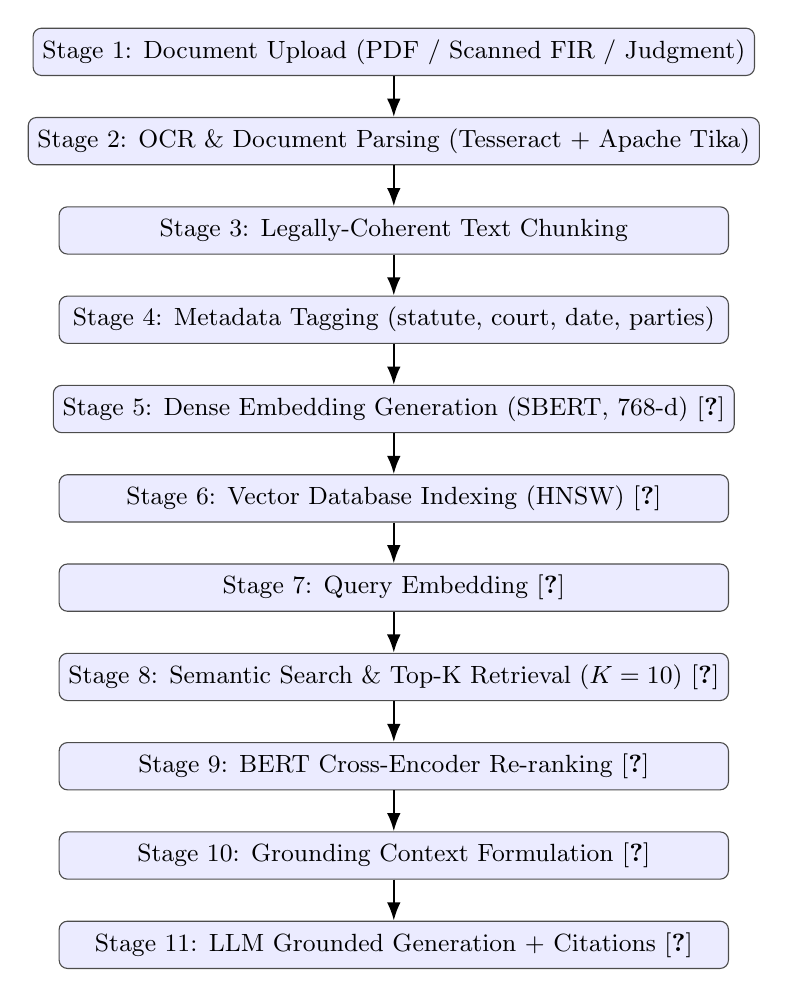
\begin{tikzpicture}[
    node distance=0.52cm,
    box/.style={rectangle, rounded corners=3pt, draw=black!70, fill=blue!8,
                minimum width=8.5cm, minimum height=0.60cm,
                font=\small, text centered},
    arrow/.style={-Latex, thick}
  ]
  \node[box] (s1)  {Stage 1: Document Upload (PDF / Scanned FIR / Judgment)};
  \node[box, below=of s1] (s2)  {Stage 2: OCR \& Document Parsing (Tesseract + Apache Tika)};
  \node[box, below=of s2] (s3)  {Stage 3: Legally-Coherent Text Chunking};
  \node[box, below=of s3] (s4)  {Stage 4: Metadata Tagging (statute, court, date, parties)};
  \node[box, below=of s4] (s5)  {Stage 5: Dense Embedding Generation (SBERT, 768-d) \cite{reimers2019sbert}};
  \node[box, below=of s5] (s6)  {Stage 6: Vector Database Indexing (HNSW) \cite{manning2008ir}};
  \node[box, below=of s6] (s7)  {Stage 7: Query Embedding \cite{reimers2019sbert}};
  \node[box, below=of s7] (s8)  {Stage 8: Semantic Search \& Top-K Retrieval ($K=10$) \cite{manning2008ir}};
  \node[box, below=of s8] (s9)  {Stage 9: BERT Cross-Encoder Re-ranking \cite{devlin2019bert}};
  \node[box, below=of s9] (s10) {Stage 10: Grounding Context Formulation \cite{lewis2020rag}};
  \node[box, below=of s10](s11) {Stage 11: LLM Grounded Generation + Citations \cite{vaswani2017attention}};

  \foreach \a/\b in {s1/s2, s2/s3, s3/s4, s4/s5, s5/s6, s6/s7,
                      s7/s8, s8/s9, s9/s10, s10/s11}
    \draw[arrow] (\a)--(\b);
\end{tikzpicture}
\caption{The Nirnay-X 11-Stage RAG Pipeline~\cite{lewis2020rag} for Indian legal document
  intelligence. Embedding uses Sentence-BERT~\cite{reimers2019sbert}; retrieval metrics
  follow Manning et al.~\cite{manning2008ir}; generation uses transformer LLMs~\cite{vaswani2017attention}.}
\label{fig:ragpipeline}
\end{figure}

\subsection{Eleven Functional Modules}

Nirnay-X exposes its capabilities through eleven integrated modules~\cite{ashley2017ai}:

\begin{enumerate}[leftmargin=*, label=\arabic*., itemsep=3pt]
  \item \textbf{RAG-Based Legal Assistant:} Context-grounded Q\&A~\cite{lewis2020rag}
    against uploaded case materials and legal corpora with mandatory source citations.
  \item \textbf{Legal Document Processing:} PDF extraction, Tesseract OCR for scanned
    files from eCourts~\cite{ecourts}, metadata tagging for structured access.
  \item \textbf{Simplified Legal Explanations:} Translation of complex statutory texts
    into plain language~\cite{vaswani2017attention} for non-lawyers, addressing the
    accessibility gap identified in the constitutional framework~\cite{const_india}.
  \item \textbf{Case Analysis \& Fact Extraction:} Automated parsing of key facts,
    dates, parties, and procedural posture using BERT-based NER~\cite{devlin2019bert}.
  \item \textbf{Legal Provision \& Precedent Retrieval:} Surfacing applicable BNS/IPC
    sections and analogous case laws via semantic search~\cite{reimers2019sbert,
    feng2022survey, cui2022survey}.
  \item \textbf{Document Summarization:} Abstractive and extractive summaries of
    lengthy judgments and petitions using transformer language
    models~\cite{vaswani2017attention, devlin2019bert}.
  \item \textbf{Semantic Search Engine:} Concept-driven search~\cite{reimers2019sbert,
    manning2008ir} across internal case documents and indexed legal statutes from
    Indian Kanoon~\cite{indiankanoon}.
  \item \textbf{Case Timeline \& Deadline Tracking:} Chronological milestones,
    limitation period tracking, and alert generation aligned with court procedure
    norms~\cite{ecourts, mlaw}.
  \item \textbf{Hearing \& Calendar Management:} Structured court calendar with
    upcoming hearing notifications sourced from eCourts data~\cite{ecourts}.
  \item \textbf{Case Organization:} Multi-case workspace structuring and client record
    linking, informed by legal practice management principles~\cite{ashley2017ai}.
  \item \textbf{Conversational Multi-Turn Interface:} Context-preserving dialogue
    interface~\cite{vaswani2017attention} supporting follow-up queries across a legal
    session, evaluated against LEGALBENCH standards~\cite{guha2023legalbench}.
\end{enumerate}

\subsection{Retrieval Strategy}

The retrieval module implements hybrid search~\cite{manning2008ir} combining:
\begin{itemize}[leftmargin=*]
  \item \textbf{Dense Retrieval:} Approximate nearest-neighbour search (HNSW index)
    on the 768-dimensional SBERT embedding space~\cite{reimers2019sbert}.
  \item \textbf{Sparse Retrieval:} BM25-based keyword matching~\cite{manning2008ir}
    on a parallel inverted index for exact statutory term retrieval.
  \item \textbf{Reciprocal Rank Fusion (RRF):} Merging dense and sparse ranked lists
    into a unified candidate set (top-20)~\cite{manning2008ir}.
  \item \textbf{Cross-Encoder Re-ranking:} A BERT-based~\cite{devlin2019bert}
    cross-encoder re-scores the top-20 candidates to produce the final top-10.
\end{itemize}

\subsection{Grounded Generation Strategy}

Nirnay-X enforces grounding~\cite{lewis2020rag} through a structured prompt template:

\begin{quote}\small\ttfamily
SYSTEM: You are a legal assistant. Answer ONLY using the provided CONTEXT.\\
Every factual claim must include a citation [DOC-\#].\\
If the answer is not in the CONTEXT, respond: ``I could not find relevant\\
information in the provided documents.''\\[4pt]
CONTEXT: [Retrieved Chunks with source labels DOC-1 through DOC-10]\\[4pt]
QUERY: [User's natural language question]
\end{quote}

This constraint ensures that responses are traceable to specific passages in the indexed
corpus, consistent with the RAG paradigm~\cite{lewis2020rag} and aligned with
verification standards assessed by LEGALBENCH~\cite{guha2023legalbench}.

\subsection{Evaluation Framework}

Nirnay-X is evaluated across three pillars, following established IR and NLP
evaluation practice~\cite{manning2008ir, guha2023legalbench}:

\subsubsection{Information Retrieval Quality~\cite{manning2008ir}}

\begin{itemize}[leftmargin=*]
  \item \textbf{Precision@K:} Proportion of the top-K retrieved chunks that are legally
    relevant. Target: P@10 $\geq$ 0.80.
  \item \textbf{Recall@K:} Proportion of all relevant passages present in the top-K
    results. Target: R@10 $\geq$ 0.85.
  \item \textbf{Mean Reciprocal Rank (MRR):} Reciprocal of the rank of the first
    correct statutory provision or precedent, averaged over all queries~\cite{manning2008ir}.
    Target: MRR $\geq$ 0.75.
  \item \textbf{NDCG@K:} Normalized Discounted Cumulative Gain with relevance
    weighting~\cite{manning2008ir}. Target: NDCG@10 $\geq$ 0.80.
\end{itemize}

\subsubsection{Generation \& Grounding Quality}

\begin{itemize}[leftmargin=*]
  \item \textbf{Faithfulness:} Proportion of generated claims supported by the
    retrieved context~\cite{lewis2020rag} (entailment classifier). Target: $\geq 0.90$.
  \item \textbf{Answer Relevance:} Degree to which the generated answer addresses the
    legal query~\cite{guha2023legalbench}. Target: $\geq 0.85$.
  \item \textbf{Context Utilization:} Proportion of retrieved context chunks
    referenced in the final response~\cite{lewis2020rag}. Target: $\geq 0.70$.
\end{itemize}

\subsubsection{Preliminary Results}

Current implementation results on a held-out Indian legal QA benchmark are summarized
in Table~\ref{tab:results}. These metrics are computed following Manning et al.'s IR
evaluation framework~\cite{manning2008ir}.

\begin{table}[H]
\centering
\caption{Preliminary Evaluation Results on Indian Legal QA Benchmark~\cite{manning2008ir}}
\label{tab:results}
\begin{tabular}{lcc}
\toprule
\textbf{Metric}          & \textbf{Current Result} & \textbf{Target} \\
\midrule
Precision@10             & 0.78                    & $\geq 0.80$     \\
Recall@10                & 0.82                    & $\geq 0.85$     \\
MRR                      & 0.71                    & $\geq 0.75$     \\
NDCG@10                  & (in progress)           & $\geq 0.80$     \\
Faithfulness             & (in progress)           & $\geq 0.90$     \\
Answer Relevance         & (in progress)           & $\geq 0.85$     \\
Context Utilization      & (in progress)           & $\geq 0.70$     \\
\bottomrule
\end{tabular}
\end{table}

\subsection{Technology Stack}

\begin{table}[H]
\centering
\caption{Nirnay-X Technology Stack}
\label{tab:techstack}
\begin{tabularx}{\textwidth}{lX}
\toprule
\textbf{Component}        & \textbf{Technology / Reference} \\
\midrule
Programming Language      & Python 3.10+ \\
LLM Framework             & LangChain / LlamaIndex~\cite{lewis2020rag} \\
Transformer Backbone      & BERT~\cite{devlin2019bert}, Attention-based LLM~\cite{vaswani2017attention} \\
Embedding Model           & Sentence-BERT (768-d)~\cite{reimers2019sbert} \\
Cross-Encoder Re-ranking  & BERT-based cross-encoder~\cite{devlin2019bert} \\
Vector Database           & Chroma / Qdrant (HNSW indexing)~\cite{manning2008ir} \\
Sparse Retrieval          & BM25 (Elasticsearch / Whoosh)~\cite{manning2008ir} \\
OCR Engine                & Tesseract OCR + Apache Tika \\
Legal Data Sources        & eCourts~\cite{ecourts}, Indian Kanoon~\cite{indiankanoon} \\
Evaluation Benchmark      & LEGALBENCH~\cite{guha2023legalbench} \\
API Layer                 & FastAPI \\
Frontend / Dashboard      & Streamlit \\
Version Control           & Git + GitHub \\
Containerization          & Docker \\
\bottomrule
\end{tabularx}
\end{table}

%% ============================================================
%% SECTION 6: EXPECTED OUTCOMES
%% ============================================================
\section{Expected Outcomes}

\subsection{End-to-End RAG System for Indian Law}

A fully functional, production-ready RAG system~\cite{lewis2020rag} capable of
ingesting diverse Indian legal documents (FIRs, judgments from eCourts~\cite{ecourts},
statutes from the Ministry of Law~\cite{mlaw}, contracts) and producing grounded,
citation-backed responses in natural language.

\subsection{Eleven Functional Modules}

All eleven platform modules~\cite{ashley2017ai} fully integrated and deployed as a
cohesive application, serving both common citizens~\cite{const_india} and legal
professionals~\cite{mlaw} from a single unified interface.

\subsection{Quantitative Evaluation Report}

A comprehensive evaluation report documenting Precision@K, Recall@K, MRR, and
NDCG~\cite{manning2008ir}, alongside response-level faithfulness and answer relevance
metrics~\cite{lewis2020rag}, on a held-out Indian legal QA benchmark. Ablation studies
will compare retrieval strategies (dense-only SBERT~\cite{reimers2019sbert} vs.\
BM25~\cite{manning2008ir} vs.\ hybrid with BERT re-ranking~\cite{devlin2019bert}).

\subsection{Legal Reasoning Benchmark Evaluation}

The system will be evaluated against LEGALBENCH~\cite{guha2023legalbench} tasks
relevant to the Indian legal domain, including issue spotting, rule application,
and statutory interpretation, providing a standard comparison point for future work
in Indian LegalTech.

\subsection{Research Publication}

A publication-quality research paper targeting:
\begin{itemize}[leftmargin=*]
  \item \textbf{Conference:} IEEE / Springer International Conference on NLP, AI
    Applications, or Legal Technology.
  \item \textbf{Journal:} Scopus / SCI-indexed journal in Knowledge-Based Systems
    or Legal Informatics.
\end{itemize}
The paper will follow IMRAD structure and compare against existing legal AI
systems~\cite{feng2022survey, cui2022survey, guha2023legalbench, indiankanoon}.

\subsection{API Documentation \& Deployment Package}

Comprehensive API documentation, a containerized deployment configuration (Docker
Compose), and a Streamlit demo dashboard illustrating the complete pipeline from
document upload~\cite{ecourts} to grounded legal response with verifiable citations.

%% ============================================================
%% SECTION 7: PROJECT PLAN
%% ============================================================
\section{Project Plan}

\subsection{Phase-Wise Project Plan}

\subsubsection{Phase 1 --- Literature Survey (Weeks 1--2)}

Survey existing research on RAG~\cite{lewis2020rag}, dense retrieval~\cite{reimers2019sbert},
transformer models~\cite{vaswani2017attention, devlin2019bert}, legal NLP~\cite{feng2022survey,
cui2022survey, ashley2017ai}, Indian legal AI~\cite{ecourts, indiankanoon}, and
legal reasoning benchmarks~\cite{guha2023legalbench}. Output: annotated bibliography.

\subsubsection{Phase 2 --- Data Collection \& Corpus Construction (Weeks 2--3)}

Collect and curate the legal corpus from eCourts~\cite{ecourts}, Indian
Kanoon~\cite{indiankanoon}, Ministry of Law statutory texts~\cite{mlaw}, BNS/IPC
statutes, BNSS/CrPC procedural texts, and anonymized FIR samples. Build the raw
legal dataset in \texttt{data/raw/}.

\subsubsection{Phase 3 --- Document Processing Pipeline (Weeks 3--4)}

Implement the ingestion pipeline: PDF parsing, Tesseract OCR for scanned documents
from eCourts~\cite{ecourts}, legally-coherent chunking~\cite{manning2008ir}, and
metadata tagging~\cite{mlaw}.

\subsubsection{Phase 4 --- Embedding \& Indexing (Week 4)}

Implement dense embedding generation using Sentence-BERT~\cite{reimers2019sbert},
vector database setup (HNSW indexing)~\cite{manning2008ir}, and BM25 sparse index
construction~\cite{manning2008ir}.

\subsubsection{Phase 5 --- Retrieval \& Re-ranking (Weeks 5--6)}

Implement semantic search~\cite{reimers2019sbert}, Reciprocal Rank Fusion~\cite{manning2008ir},
and BERT-based cross-encoder re-ranking~\cite{devlin2019bert}. Conduct retrieval
ablation studies.

\subsubsection{Phase 6 --- Grounded Generation (Week 6)}

Implement the grounding prompt framework~\cite{lewis2020rag} with citation-token
enforcement. Integrate transformer-based LLM inference~\cite{vaswani2017attention}
with constrained decoding.

\subsubsection{Phase 7 --- Module Integration (Weeks 7--8)}

Integrate all eleven functional modules~\cite{ashley2017ai} into the unified Nirnay-X
application. Build the FastAPI backend and Streamlit frontend.

\subsubsection{Phase 8 --- Evaluation \& Benchmarking (Weeks 8--9)}

Run the complete evaluation suite using IR metrics~\cite{manning2008ir} and
LEGALBENCH-inspired tasks~\cite{guha2023legalbench}. Conduct legal QA comparison
against Indian Kanoon~\cite{indiankanoon}. Log all results to \texttt{results/}.

\subsubsection{Phase 9 --- Beta Testing with Legal Stakeholders (Week 9)}

Conduct user testing with legal professionals and non-lawyer users. Collect structured
feedback on usability, response quality, and citation utility.

\subsubsection{Phase 10 --- Research Paper \& Final Documentation (Week 10)}

Prepare the full research paper (IMRAD format), finalize API documentation, complete
the Streamlit demo dashboard, and submit all deliverables.

\subsection{Timeline Summary}

\begin{table}[H]
\centering
\caption{10-Week Project Timeline}
\label{tab:timeline}
\begin{tabular}{cll}
\toprule
\textbf{Weeks} & \textbf{Phase} & \textbf{Key Deliverable} \\
\midrule
1--2  & Literature Survey~\cite{lewis2020rag,reimers2019sbert,guha2023legalbench}
      & Annotated bibliography; baselines identified \\
2--3  & Data Collection~\cite{ecourts,indiankanoon,mlaw}
      & Legal corpus assembled in \texttt{data/raw/} \\
3--4  & Document Processing Pipeline~\cite{manning2008ir}
      & Ingestion pipeline operational \\
4     & Embedding \& Indexing~\cite{reimers2019sbert,manning2008ir}
      & Vector database populated \\
5--6  & Retrieval \& Re-ranking~\cite{devlin2019bert,manning2008ir}
      & Retrieval ablation results \\
6     & Grounded Generation~\cite{lewis2020rag,vaswani2017attention}
      & Citation-constrained LLM integrated \\
7--8  & Module Integration~\cite{ashley2017ai}
      & All 11 modules integrated \\
8--9  & Evaluation \& Benchmarking~\cite{manning2008ir,guha2023legalbench}
      & Full evaluation report \\
9     & Beta Testing & User feedback report \\
10    & Paper \& Documentation~\cite{feng2022survey,cui2022survey}
      & Submission-ready manuscript \\
\bottomrule
\end{tabular}
\end{table}

\subsection{Final Deliverables}

\begin{enumerate}[leftmargin=*, label=\arabic*.]
  \item Fully integrated Nirnay-X RAG application~\cite{lewis2020rag} with all
    11 modules~\cite{ashley2017ai}
  \item Comprehensive evaluation report with IR metrics~\cite{manning2008ir}
    and ablation studies
  \item Legal reasoning evaluation against LEGALBENCH~\cite{guha2023legalbench}
    and Indian Kanoon~\cite{indiankanoon}
  \item API documentation and usage examples (\texttt{docs/})
  \item Containerized deployment package (Docker Compose)
  \item Interactive Streamlit demonstration dashboard
  \item Publication-quality research paper (IEEE / Springer target), grounded in
    the literature surveyed~\cite{lewis2020rag, vaswani2017attention, reimers2019sbert,
    devlin2019bert, feng2022survey, ashley2017ai, guha2023legalbench}
\end{enumerate}

%% ============================================================
%% REFERENCES
%% ============================================================
\newpage
\begin{thebibliography}{99}

%% -- Core RAG & NLP --
\bibitem{lewis2020rag}
P.~Lewis, E.~Perez, A.~Piktus, et al.,
``Retrieval-Augmented Generation for Knowledge-Intensive NLP Tasks,''
\textit{Advances in Neural Information Processing Systems (NeurIPS)},
vol.~33, pp.~9459--9474, 2020.
\url{https://arxiv.org/abs/2005.11401}

\bibitem{vaswani2017attention}
A.~Vaswani, N.~Shazeer, N.~Parmar, et al.,
``Attention Is All You Need,''
\textit{Advances in Neural Information Processing Systems (NeurIPS)},
vol.~30, pp.~5998--6008, 2017.
\url{https://arxiv.org/abs/1706.03762}

\bibitem{reimers2019sbert}
N.~Reimers and I.~Gurevych,
``Sentence-BERT: Sentence Embeddings using Siamese BERT-Networks,''
\textit{Proceedings of EMNLP-IJCNLP}, pp.~3982--3992, 2019.
\url{https://arxiv.org/abs/1908.10084}

\bibitem{devlin2019bert}
J.~Devlin, M.-W.~Chang, K.~Lee, and K.~Toutanova,
``BERT: Pre-training of Deep Bidirectional Transformers for Language Understanding,''
\textit{Proceedings of NAACL-HLT}, pp.~4171--4186, 2019.
\url{https://arxiv.org/abs/1810.04805}

%% -- Information Retrieval --
\bibitem{manning2008ir}
C.~D.~Manning, P.~Raghavan, and H.~Sch\"{u}tze,
\textit{Introduction to Information Retrieval}.
Cambridge University Press, 2008.
\url{https://nlp.stanford.edu/IR-book/}

%% -- Legal NLP & AI --
\bibitem{feng2022survey}
Y.~Feng, C.~Li, and V.~Ng,
``Legal Judgment Prediction: A Survey of the State of the Art,''
\textit{Proceedings of the 31st International Joint Conference on Artificial
Intelligence (IJCAI)}, pp.~5461--5469, 2022.

\bibitem{cui2022survey}
J.~Cui, X.~Shen, F.~Nie, Z.~Wang, J.~Wang, and Y.~Chen,
``A Survey on Legal Judgment Prediction: Datasets, Metrics, Models, and Challenges,''
2022.
\url{https://arxiv.org/abs/2204.04185}

\bibitem{guha2023legalbench}
N.~Guha, J.~Nyarko, D.~Ho, et al.,
``LEGALBENCH: A Collaboratively Built Benchmark for Measuring Legal Reasoning in
Large Language Models,''
\textit{Advances in Neural Information Processing Systems (NeurIPS)}, 2023.
\url{https://arxiv.org/abs/2308.11462}

\bibitem{ashley2017ai}
K.~D.~Ashley,
\textit{Artificial Intelligence and Legal Analytics}.
Cambridge University Press, 2017.

%% -- Indian Legal Infrastructure --
\bibitem{ecourts}
e-Committee, Supreme Court of India,
``Judgements and Orders of the Supreme Court and High Courts of India,''
\textit{eCourts Services}, Government of India.
\url{https://ecourts.gov.in}

\bibitem{indiankanoon}
Indian Kanoon,
``Prism -- AI-Powered Legal Research Assistant.''
\url{https://indiankanoon.org}

\bibitem{mlaw}
Ministry of Law and Justice, Government of India.
\url{https://lawmin.gov.in}

%% -- Constitutional Framework --
\bibitem{const_india}
Constitution of India, Article~39A: Equal Justice and Free Legal Aid.
Government of India, 1949 (as amended).
\url{https://legislative.gov.in/constitution-of-india/}

\end{thebibliography}

\end{document}
